% 附錄 A 第 4 段：A.12–A.14（動畫 M12–M14，MIT 18.212 L4）
% 圖由 mit/make_figs_part4.py 產生（含數字檢查）；格子 (i,j) = 第 i 列第 j 行，1 起算。
% figs_part4.tex —— 由 mit/make_figs_part4.py 產生，請勿手動修改。
% 重新產生：python mit/make_figs_part4.py（附錄 A.12–A.14，動畫 M12–M14）

\newcommand{\FigMXIIConvert}{%
\begin{tikzpicture}
\fill[cLeft!20] (0,0) -- (0.62,0) -- (0.62,-0.62) -- (0,-0.62) -- cycle;
\fill[cLeft!20] (0.62,0) -- (1.24,0) -- (1.24,-0.62) -- (0.62,-0.62) -- cycle;
\fill[cLeft!20] (1.24,0) -- (1.86,0) -- (1.86,-0.62) -- (1.24,-0.62) -- cycle;
\fill[cRight!18] (0,-0.62) -- (0.62,-0.62) -- (0.62,-1.24) -- (0,-1.24) -- cycle;
\fill[cRight!18] (0.62,-0.62) -- (1.24,-0.62) -- (1.24,-1.24) -- (0.62,-1.24) -- cycle;
\fill[cRight!18] (1.24,-0.62) -- (1.86,-0.62) -- (1.86,-1.24) -- (1.24,-1.24) -- cycle;
\draw[gray!70!black,line width=0.5pt] (0,0) -- (0.62,0) -- (0.62,-0.62) -- (0,-0.62) -- cycle;
\draw[gray!70!black,line width=0.5pt] (0.62,0) -- (1.24,0) -- (1.24,-0.62) -- (0.62,-0.62) -- cycle;
\draw[gray!70!black,line width=0.5pt] (1.24,0) -- (1.86,0) -- (1.86,-0.62) -- (1.24,-0.62) -- cycle;
\draw[gray!70!black,line width=0.5pt] (0,-0.62) -- (0.62,-0.62) -- (0.62,-1.24) -- (0,-1.24) -- cycle;
\draw[gray!70!black,line width=0.5pt] (0.62,-0.62) -- (1.24,-0.62) -- (1.24,-1.24) -- (0.62,-1.24) -- cycle;
\draw[gray!70!black,line width=0.5pt] (1.24,-0.62) -- (1.86,-0.62) -- (1.86,-1.24) -- (1.24,-1.24) -- cycle;
\node[font=\small,inner sep=0pt] at (0.31,-0.31) {$1$};
\node[font=\small,inner sep=0pt] at (0.93,-0.31) {$2$};
\node[font=\small,inner sep=0pt] at (1.55,-0.31) {$4$};
\node[font=\small,inner sep=0pt] at (0.31,-0.93) {$3$};
\node[font=\small,inner sep=0pt] at (0.93,-0.93) {$5$};
\node[font=\small,inner sep=0pt] at (1.55,-0.93) {$6$};
\node[anchor=west,font=\small,text=cLeft] at (1.98,-0.31) {$\to\mathrm{U}$};
\node[anchor=west,font=\small,text=cRight] at (1.98,-0.93) {$\to\mathrm{D}$};
\draw[-{Stealth[length=5pt]},gray!60!black,line width=0.7pt] (3.1,-0.62) -- (4,-0.62);
\draw[gray!55,line width=0.4pt] (4.35,-0.9) -- (7.11,-0.9);
\draw[cLeft,line width=1.5pt,line cap=round] (4.35,-0.9) -- (4.81,-0.44);
\draw[cLeft,line width=1.5pt,line cap=round] (4.81,-0.44) -- (5.27,0.02);
\draw[cRight,line width=1.5pt,line cap=round] (5.27,0.02) -- (5.73,-0.44);
\draw[cLeft,line width=1.5pt,line cap=round] (5.73,-0.44) -- (6.19,0.02);
\draw[cRight,line width=1.5pt,line cap=round] (6.19,0.02) -- (6.65,-0.44);
\draw[cRight,line width=1.5pt,line cap=round] (6.65,-0.44) -- (7.11,-0.9);
\fill[black] (4.35,-0.9) circle (0.035);
\fill[black] (4.81,-0.44) circle (0.035);
\fill[black] (5.27,0.02) circle (0.035);
\fill[black] (5.73,-0.44) circle (0.035);
\fill[black] (6.19,0.02) circle (0.035);
\fill[black] (6.65,-0.44) circle (0.035);
\fill[black] (7.11,-0.9) circle (0.035);
\node[font=\scriptsize,text=gray!70!black] at (4.58,-1.14) {1};
\node[font=\small,text=cLeft] at (4.58,-1.46) {$\mathrm{U}$};
\node[font=\scriptsize,text=gray!70!black] at (5.04,-1.14) {2};
\node[font=\small,text=cLeft] at (5.04,-1.46) {$\mathrm{U}$};
\node[font=\scriptsize,text=gray!70!black] at (5.5,-1.14) {3};
\node[font=\small,text=cRight] at (5.5,-1.46) {$\mathrm{D}$};
\node[font=\scriptsize,text=gray!70!black] at (5.96,-1.14) {4};
\node[font=\small,text=cLeft] at (5.96,-1.46) {$\mathrm{U}$};
\node[font=\scriptsize,text=gray!70!black] at (6.42,-1.14) {5};
\node[font=\small,text=cRight] at (6.42,-1.46) {$\mathrm{D}$};
\node[font=\scriptsize,text=gray!70!black] at (6.88,-1.14) {6};
\node[font=\small,text=cRight] at (6.88,-1.46) {$\mathrm{D}$};
\node[anchor=east,font=\scriptsize,text=gray!70!black] at (4.05,-1.14) {步};
\end{tikzpicture}}

\newcommand{\FigMXIIAll}{%
\begin{tikzpicture}
\fill[cLeft!20] (-0.51,0) -- (-0.17,0) -- (-0.17,-0.34) -- (-0.51,-0.34) -- cycle;
\fill[cLeft!20] (-0.17,0) -- (0.17,0) -- (0.17,-0.34) -- (-0.17,-0.34) -- cycle;
\fill[cLeft!20] (0.17,0) -- (0.51,0) -- (0.51,-0.34) -- (0.17,-0.34) -- cycle;
\fill[cRight!18] (-0.51,-0.34) -- (-0.17,-0.34) -- (-0.17,-0.68) -- (-0.51,-0.68) -- cycle;
\fill[cRight!18] (-0.17,-0.34) -- (0.17,-0.34) -- (0.17,-0.68) -- (-0.17,-0.68) -- cycle;
\fill[cRight!18] (0.17,-0.34) -- (0.51,-0.34) -- (0.51,-0.68) -- (0.17,-0.68) -- cycle;
\draw[gray!70!black,line width=0.5pt] (-0.51,0) -- (-0.17,0) -- (-0.17,-0.34) -- (-0.51,-0.34) -- cycle;
\draw[gray!70!black,line width=0.5pt] (-0.17,0) -- (0.17,0) -- (0.17,-0.34) -- (-0.17,-0.34) -- cycle;
\draw[gray!70!black,line width=0.5pt] (0.17,0) -- (0.51,0) -- (0.51,-0.34) -- (0.17,-0.34) -- cycle;
\draw[gray!70!black,line width=0.5pt] (-0.51,-0.34) -- (-0.17,-0.34) -- (-0.17,-0.68) -- (-0.51,-0.68) -- cycle;
\draw[gray!70!black,line width=0.5pt] (-0.17,-0.34) -- (0.17,-0.34) -- (0.17,-0.68) -- (-0.17,-0.68) -- cycle;
\draw[gray!70!black,line width=0.5pt] (0.17,-0.34) -- (0.51,-0.34) -- (0.51,-0.68) -- (0.17,-0.68) -- cycle;
\node[font=\scriptsize,inner sep=0pt] at (-0.34,-0.17) {$1$};
\node[font=\scriptsize,inner sep=0pt] at (0,-0.17) {$2$};
\node[font=\scriptsize,inner sep=0pt] at (0.34,-0.17) {$3$};
\node[font=\scriptsize,inner sep=0pt] at (-0.34,-0.51) {$4$};
\node[font=\scriptsize,inner sep=0pt] at (0,-0.51) {$5$};
\node[font=\scriptsize,inner sep=0pt] at (0.34,-0.51) {$6$};
\node[font=\small,text=gray!60!black] at (0,-0.98) {$\downarrow$};
\draw[gray!55,line width=0.4pt] (-0.6,-1.9) -- (0.6,-1.9);
\draw[cLeft,line width=1.2pt,line cap=round] (-0.6,-1.9) -- (-0.4,-1.7);
\draw[cLeft,line width=1.2pt,line cap=round] (-0.4,-1.7) -- (-0.2,-1.5);
\draw[cLeft,line width=1.2pt,line cap=round] (-0.2,-1.5) -- (0,-1.3);
\draw[cRight,line width=1.2pt,line cap=round] (0,-1.3) -- (0.2,-1.5);
\draw[cRight,line width=1.2pt,line cap=round] (0.2,-1.5) -- (0.4,-1.7);
\draw[cRight,line width=1.2pt,line cap=round] (0.4,-1.7) -- (0.6,-1.9);
\node[font=\scriptsize] at (0,-2.16) {$\mathrm{UUUDDD}$};
\fill[cLeft!20] (1.74,0) -- (2.08,0) -- (2.08,-0.34) -- (1.74,-0.34) -- cycle;
\fill[cLeft!20] (2.08,0) -- (2.42,0) -- (2.42,-0.34) -- (2.08,-0.34) -- cycle;
\fill[cLeft!20] (2.42,0) -- (2.76,0) -- (2.76,-0.34) -- (2.42,-0.34) -- cycle;
\fill[cRight!18] (1.74,-0.34) -- (2.08,-0.34) -- (2.08,-0.68) -- (1.74,-0.68) -- cycle;
\fill[cRight!18] (2.08,-0.34) -- (2.42,-0.34) -- (2.42,-0.68) -- (2.08,-0.68) -- cycle;
\fill[cRight!18] (2.42,-0.34) -- (2.76,-0.34) -- (2.76,-0.68) -- (2.42,-0.68) -- cycle;
\draw[gray!70!black,line width=0.5pt] (1.74,0) -- (2.08,0) -- (2.08,-0.34) -- (1.74,-0.34) -- cycle;
\draw[gray!70!black,line width=0.5pt] (2.08,0) -- (2.42,0) -- (2.42,-0.34) -- (2.08,-0.34) -- cycle;
\draw[gray!70!black,line width=0.5pt] (2.42,0) -- (2.76,0) -- (2.76,-0.34) -- (2.42,-0.34) -- cycle;
\draw[gray!70!black,line width=0.5pt] (1.74,-0.34) -- (2.08,-0.34) -- (2.08,-0.68) -- (1.74,-0.68) -- cycle;
\draw[gray!70!black,line width=0.5pt] (2.08,-0.34) -- (2.42,-0.34) -- (2.42,-0.68) -- (2.08,-0.68) -- cycle;
\draw[gray!70!black,line width=0.5pt] (2.42,-0.34) -- (2.76,-0.34) -- (2.76,-0.68) -- (2.42,-0.68) -- cycle;
\node[font=\scriptsize,inner sep=0pt] at (1.91,-0.17) {$1$};
\node[font=\scriptsize,inner sep=0pt] at (2.25,-0.17) {$2$};
\node[font=\scriptsize,inner sep=0pt] at (2.59,-0.17) {$4$};
\node[font=\scriptsize,inner sep=0pt] at (1.91,-0.51) {$3$};
\node[font=\scriptsize,inner sep=0pt] at (2.25,-0.51) {$5$};
\node[font=\scriptsize,inner sep=0pt] at (2.59,-0.51) {$6$};
\node[font=\small,text=gray!60!black] at (2.25,-0.98) {$\downarrow$};
\draw[gray!55,line width=0.4pt] (1.65,-1.9) -- (2.85,-1.9);
\draw[cLeft,line width=1.2pt,line cap=round] (1.65,-1.9) -- (1.85,-1.7);
\draw[cLeft,line width=1.2pt,line cap=round] (1.85,-1.7) -- (2.05,-1.5);
\draw[cRight,line width=1.2pt,line cap=round] (2.05,-1.5) -- (2.25,-1.7);
\draw[cLeft,line width=1.2pt,line cap=round] (2.25,-1.7) -- (2.45,-1.5);
\draw[cRight,line width=1.2pt,line cap=round] (2.45,-1.5) -- (2.65,-1.7);
\draw[cRight,line width=1.2pt,line cap=round] (2.65,-1.7) -- (2.85,-1.9);
\node[font=\scriptsize] at (2.25,-2.16) {$\mathrm{UUDUDD}$};
\draw[cTop,dashed,line width=0.7pt,rounded corners=3pt] (1.4,0.14) rectangle (3.1,-2.38);
\fill[cLeft!20] (3.99,0) -- (4.33,0) -- (4.33,-0.34) -- (3.99,-0.34) -- cycle;
\fill[cLeft!20] (4.33,0) -- (4.67,0) -- (4.67,-0.34) -- (4.33,-0.34) -- cycle;
\fill[cLeft!20] (4.67,0) -- (5.01,0) -- (5.01,-0.34) -- (4.67,-0.34) -- cycle;
\fill[cRight!18] (3.99,-0.34) -- (4.33,-0.34) -- (4.33,-0.68) -- (3.99,-0.68) -- cycle;
\fill[cRight!18] (4.33,-0.34) -- (4.67,-0.34) -- (4.67,-0.68) -- (4.33,-0.68) -- cycle;
\fill[cRight!18] (4.67,-0.34) -- (5.01,-0.34) -- (5.01,-0.68) -- (4.67,-0.68) -- cycle;
\draw[gray!70!black,line width=0.5pt] (3.99,0) -- (4.33,0) -- (4.33,-0.34) -- (3.99,-0.34) -- cycle;
\draw[gray!70!black,line width=0.5pt] (4.33,0) -- (4.67,0) -- (4.67,-0.34) -- (4.33,-0.34) -- cycle;
\draw[gray!70!black,line width=0.5pt] (4.67,0) -- (5.01,0) -- (5.01,-0.34) -- (4.67,-0.34) -- cycle;
\draw[gray!70!black,line width=0.5pt] (3.99,-0.34) -- (4.33,-0.34) -- (4.33,-0.68) -- (3.99,-0.68) -- cycle;
\draw[gray!70!black,line width=0.5pt] (4.33,-0.34) -- (4.67,-0.34) -- (4.67,-0.68) -- (4.33,-0.68) -- cycle;
\draw[gray!70!black,line width=0.5pt] (4.67,-0.34) -- (5.01,-0.34) -- (5.01,-0.68) -- (4.67,-0.68) -- cycle;
\node[font=\scriptsize,inner sep=0pt] at (4.16,-0.17) {$1$};
\node[font=\scriptsize,inner sep=0pt] at (4.5,-0.17) {$2$};
\node[font=\scriptsize,inner sep=0pt] at (4.84,-0.17) {$5$};
\node[font=\scriptsize,inner sep=0pt] at (4.16,-0.51) {$3$};
\node[font=\scriptsize,inner sep=0pt] at (4.5,-0.51) {$4$};
\node[font=\scriptsize,inner sep=0pt] at (4.84,-0.51) {$6$};
\node[font=\small,text=gray!60!black] at (4.5,-0.98) {$\downarrow$};
\draw[gray!55,line width=0.4pt] (3.9,-1.9) -- (5.1,-1.9);
\draw[cLeft,line width=1.2pt,line cap=round] (3.9,-1.9) -- (4.1,-1.7);
\draw[cLeft,line width=1.2pt,line cap=round] (4.1,-1.7) -- (4.3,-1.5);
\draw[cRight,line width=1.2pt,line cap=round] (4.3,-1.5) -- (4.5,-1.7);
\draw[cRight,line width=1.2pt,line cap=round] (4.5,-1.7) -- (4.7,-1.9);
\draw[cLeft,line width=1.2pt,line cap=round] (4.7,-1.9) -- (4.9,-1.7);
\draw[cRight,line width=1.2pt,line cap=round] (4.9,-1.7) -- (5.1,-1.9);
\node[font=\scriptsize] at (4.5,-2.16) {$\mathrm{UUDDUD}$};
\fill[cLeft!20] (6.24,0) -- (6.58,0) -- (6.58,-0.34) -- (6.24,-0.34) -- cycle;
\fill[cLeft!20] (6.58,0) -- (6.92,0) -- (6.92,-0.34) -- (6.58,-0.34) -- cycle;
\fill[cLeft!20] (6.92,0) -- (7.26,0) -- (7.26,-0.34) -- (6.92,-0.34) -- cycle;
\fill[cRight!18] (6.24,-0.34) -- (6.58,-0.34) -- (6.58,-0.68) -- (6.24,-0.68) -- cycle;
\fill[cRight!18] (6.58,-0.34) -- (6.92,-0.34) -- (6.92,-0.68) -- (6.58,-0.68) -- cycle;
\fill[cRight!18] (6.92,-0.34) -- (7.26,-0.34) -- (7.26,-0.68) -- (6.92,-0.68) -- cycle;
\draw[gray!70!black,line width=0.5pt] (6.24,0) -- (6.58,0) -- (6.58,-0.34) -- (6.24,-0.34) -- cycle;
\draw[gray!70!black,line width=0.5pt] (6.58,0) -- (6.92,0) -- (6.92,-0.34) -- (6.58,-0.34) -- cycle;
\draw[gray!70!black,line width=0.5pt] (6.92,0) -- (7.26,0) -- (7.26,-0.34) -- (6.92,-0.34) -- cycle;
\draw[gray!70!black,line width=0.5pt] (6.24,-0.34) -- (6.58,-0.34) -- (6.58,-0.68) -- (6.24,-0.68) -- cycle;
\draw[gray!70!black,line width=0.5pt] (6.58,-0.34) -- (6.92,-0.34) -- (6.92,-0.68) -- (6.58,-0.68) -- cycle;
\draw[gray!70!black,line width=0.5pt] (6.92,-0.34) -- (7.26,-0.34) -- (7.26,-0.68) -- (6.92,-0.68) -- cycle;
\node[font=\scriptsize,inner sep=0pt] at (6.41,-0.17) {$1$};
\node[font=\scriptsize,inner sep=0pt] at (6.75,-0.17) {$3$};
\node[font=\scriptsize,inner sep=0pt] at (7.09,-0.17) {$4$};
\node[font=\scriptsize,inner sep=0pt] at (6.41,-0.51) {$2$};
\node[font=\scriptsize,inner sep=0pt] at (6.75,-0.51) {$5$};
\node[font=\scriptsize,inner sep=0pt] at (7.09,-0.51) {$6$};
\node[font=\small,text=gray!60!black] at (6.75,-0.98) {$\downarrow$};
\draw[gray!55,line width=0.4pt] (6.15,-1.9) -- (7.35,-1.9);
\draw[cLeft,line width=1.2pt,line cap=round] (6.15,-1.9) -- (6.35,-1.7);
\draw[cRight,line width=1.2pt,line cap=round] (6.35,-1.7) -- (6.55,-1.9);
\draw[cLeft,line width=1.2pt,line cap=round] (6.55,-1.9) -- (6.75,-1.7);
\draw[cLeft,line width=1.2pt,line cap=round] (6.75,-1.7) -- (6.95,-1.5);
\draw[cRight,line width=1.2pt,line cap=round] (6.95,-1.5) -- (7.15,-1.7);
\draw[cRight,line width=1.2pt,line cap=round] (7.15,-1.7) -- (7.35,-1.9);
\node[font=\scriptsize] at (6.75,-2.16) {$\mathrm{UDUUDD}$};
\fill[cLeft!20] (8.49,0) -- (8.83,0) -- (8.83,-0.34) -- (8.49,-0.34) -- cycle;
\fill[cLeft!20] (8.83,0) -- (9.17,0) -- (9.17,-0.34) -- (8.83,-0.34) -- cycle;
\fill[cLeft!20] (9.17,0) -- (9.51,0) -- (9.51,-0.34) -- (9.17,-0.34) -- cycle;
\fill[cRight!18] (8.49,-0.34) -- (8.83,-0.34) -- (8.83,-0.68) -- (8.49,-0.68) -- cycle;
\fill[cRight!18] (8.83,-0.34) -- (9.17,-0.34) -- (9.17,-0.68) -- (8.83,-0.68) -- cycle;
\fill[cRight!18] (9.17,-0.34) -- (9.51,-0.34) -- (9.51,-0.68) -- (9.17,-0.68) -- cycle;
\draw[gray!70!black,line width=0.5pt] (8.49,0) -- (8.83,0) -- (8.83,-0.34) -- (8.49,-0.34) -- cycle;
\draw[gray!70!black,line width=0.5pt] (8.83,0) -- (9.17,0) -- (9.17,-0.34) -- (8.83,-0.34) -- cycle;
\draw[gray!70!black,line width=0.5pt] (9.17,0) -- (9.51,0) -- (9.51,-0.34) -- (9.17,-0.34) -- cycle;
\draw[gray!70!black,line width=0.5pt] (8.49,-0.34) -- (8.83,-0.34) -- (8.83,-0.68) -- (8.49,-0.68) -- cycle;
\draw[gray!70!black,line width=0.5pt] (8.83,-0.34) -- (9.17,-0.34) -- (9.17,-0.68) -- (8.83,-0.68) -- cycle;
\draw[gray!70!black,line width=0.5pt] (9.17,-0.34) -- (9.51,-0.34) -- (9.51,-0.68) -- (9.17,-0.68) -- cycle;
\node[font=\scriptsize,inner sep=0pt] at (8.66,-0.17) {$1$};
\node[font=\scriptsize,inner sep=0pt] at (9,-0.17) {$3$};
\node[font=\scriptsize,inner sep=0pt] at (9.34,-0.17) {$5$};
\node[font=\scriptsize,inner sep=0pt] at (8.66,-0.51) {$2$};
\node[font=\scriptsize,inner sep=0pt] at (9,-0.51) {$4$};
\node[font=\scriptsize,inner sep=0pt] at (9.34,-0.51) {$6$};
\node[font=\small,text=gray!60!black] at (9,-0.98) {$\downarrow$};
\draw[gray!55,line width=0.4pt] (8.4,-1.9) -- (9.6,-1.9);
\draw[cLeft,line width=1.2pt,line cap=round] (8.4,-1.9) -- (8.6,-1.7);
\draw[cRight,line width=1.2pt,line cap=round] (8.6,-1.7) -- (8.8,-1.9);
\draw[cLeft,line width=1.2pt,line cap=round] (8.8,-1.9) -- (9,-1.7);
\draw[cRight,line width=1.2pt,line cap=round] (9,-1.7) -- (9.2,-1.9);
\draw[cLeft,line width=1.2pt,line cap=round] (9.2,-1.9) -- (9.4,-1.7);
\draw[cRight,line width=1.2pt,line cap=round] (9.4,-1.7) -- (9.6,-1.9);
\node[font=\scriptsize] at (9,-2.16) {$\mathrm{UDUDUD}$};
\end{tikzpicture}}

\newcommand{\FigMXIIGenGood}{%
\begin{tikzpicture}[baseline={(0,-0.63)}]
\fill[cLeft!20] (0,0) -- (0.36,0) -- (0.36,-0.36) -- (0,-0.36) -- cycle;
\fill[cLeft!20] (0.36,0) -- (0.72,0) -- (0.72,-0.36) -- (0.36,-0.36) -- cycle;
\fill[cRight!18] (0,-0.36) -- (0.36,-0.36) -- (0.36,-0.72) -- (0,-0.72) -- cycle;
\fill[cRight!18] (0.36,-0.36) -- (0.72,-0.36) -- (0.72,-0.72) -- (0.36,-0.72) -- cycle;
\fill[olive!22] (0,-0.72) -- (0.36,-0.72) -- (0.36,-1.08) -- (0,-1.08) -- cycle;
\draw[gray!70!black,line width=0.5pt] (0,0) -- (0.36,0) -- (0.36,-0.36) -- (0,-0.36) -- cycle;
\draw[gray!70!black,line width=0.5pt] (0.36,0) -- (0.72,0) -- (0.72,-0.36) -- (0.36,-0.36) -- cycle;
\draw[gray!70!black,line width=0.5pt] (0,-0.36) -- (0.36,-0.36) -- (0.36,-0.72) -- (0,-0.72) -- cycle;
\draw[gray!70!black,line width=0.5pt] (0.36,-0.36) -- (0.72,-0.36) -- (0.72,-0.72) -- (0.36,-0.72) -- cycle;
\draw[gray!70!black,line width=0.5pt] (0,-0.72) -- (0.36,-0.72) -- (0.36,-1.08) -- (0,-1.08) -- cycle;
\node[font=\footnotesize,inner sep=0pt] at (0.18,-0.18) {$1$};
\node[font=\footnotesize,inner sep=0pt] at (0.54,-0.18) {$3$};
\node[font=\footnotesize,inner sep=0pt] at (0.18,-0.54) {$2$};
\node[font=\footnotesize,inner sep=0pt] at (0.54,-0.54) {$5$};
\node[font=\footnotesize,inner sep=0pt] at (0.18,-0.9) {$4$};
\path (-0.05,0.14) rectangle (0.77,-1.22);
\end{tikzpicture}}

\newcommand{\FigMXIIGenBad}{%
\begin{tikzpicture}[baseline={(0,-0.63)}]
\fill[cLeft!20] (0,0) -- (0.36,0) -- (0.36,-0.36) -- (0,-0.36) -- cycle;
\fill[cLeft!20] (0.36,0) -- (0.72,0) -- (0.72,-0.36) -- (0.36,-0.36) -- cycle;
\fill[cRight!18] (0,-0.36) -- (0.36,-0.36) -- (0.36,-0.72) -- (0,-0.72) -- cycle;
\fill[cRight!18] (0.36,-0.36) -- (0.72,-0.36) -- (0.72,-0.72) -- (0.36,-0.72) -- cycle;
\fill[olive!22] (0,-0.72) -- (0.36,-0.72) -- (0.36,-1.08) -- (0,-1.08) -- cycle;
\draw[gray!70!black,line width=0.5pt] (0,0) -- (0.36,0) -- (0.36,-0.36) -- (0,-0.36) -- cycle;
\draw[gray!70!black,line width=0.5pt] (0.36,0) -- (0.72,0) -- (0.72,-0.36) -- (0.36,-0.36) -- cycle;
\draw[gray!70!black,line width=0.5pt] (0,-0.36) -- (0.36,-0.36) -- (0.36,-0.72) -- (0,-0.72) -- cycle;
\draw[gray!70!black,line width=0.5pt] (0.36,-0.36) -- (0.72,-0.36) -- (0.72,-0.72) -- (0.36,-0.72) -- cycle;
\draw[gray!70!black,line width=0.5pt] (0,-0.72) -- (0.36,-0.72) -- (0.36,-1.08) -- (0,-1.08) -- cycle;
\node[font=\footnotesize,inner sep=0pt] at (0.18,-0.18) {$1$};
\node[font=\footnotesize,inner sep=0pt,text=cBad] at (0.54,-0.18) {$5$};
\node[font=\footnotesize,inner sep=0pt] at (0.18,-0.54) {$2$};
\node[font=\footnotesize,inner sep=0pt,text=cBad] at (0.54,-0.54) {$4$};
\node[font=\footnotesize,inner sep=0pt] at (0.18,-0.9) {$3$};
\draw[cBad,line width=1pt] (0.36,0) rectangle (0.72,-0.72);
\path (-0.05,0.14) rectangle (0.77,-1.22);
\end{tikzpicture}}

\newcommand{\FigMXIIIHook}{%
\begin{tikzpicture}
\fill[yellow!55] (1.24,0) -- (1.86,0) -- (1.86,-0.62) -- (1.24,-0.62) -- cycle;
\fill[yellow!55] (1.86,0) -- (2.48,0) -- (2.48,-0.62) -- (1.86,-0.62) -- cycle;
\fill[yellow!55] (0.62,-0.62) -- (1.24,-0.62) -- (1.24,-1.24) -- (0.62,-1.24) -- cycle;
\fill[cTop!45] (0.62,0) -- (1.24,0) -- (1.24,-0.62) -- (0.62,-0.62) -- cycle;
\draw[gray!70!black,line width=0.5pt] (0,0) -- (0.62,0) -- (0.62,-0.62) -- (0,-0.62) -- cycle;
\draw[gray!70!black,line width=0.5pt] (0.62,0) -- (1.24,0) -- (1.24,-0.62) -- (0.62,-0.62) -- cycle;
\draw[gray!70!black,line width=0.5pt] (1.24,0) -- (1.86,0) -- (1.86,-0.62) -- (1.24,-0.62) -- cycle;
\draw[gray!70!black,line width=0.5pt] (1.86,0) -- (2.48,0) -- (2.48,-0.62) -- (1.86,-0.62) -- cycle;
\draw[gray!70!black,line width=0.5pt] (0,-0.62) -- (0.62,-0.62) -- (0.62,-1.24) -- (0,-1.24) -- cycle;
\draw[gray!70!black,line width=0.5pt] (0.62,-0.62) -- (1.24,-0.62) -- (1.24,-1.24) -- (0.62,-1.24) -- cycle;
\draw[gray!70!black,line width=0.5pt] (1.24,-0.62) -- (1.86,-0.62) -- (1.86,-1.24) -- (1.24,-1.24) -- cycle;
\draw[gray!70!black,line width=0.5pt] (0,-1.24) -- (0.62,-1.24) -- (0.62,-1.86) -- (0,-1.86) -- cycle;
\node[font=\small] at (0.93,-0.31) {$c$};
\draw[orange!70!black,line width=0.6pt] (1.3,0.1) -- (1.3,0.2) -- (2.42,0.2) -- (2.42,0.1);
\node[font=\footnotesize,text=orange!70!black] at (1.86,0.43) {臂};
\draw[orange!70!black,line width=0.6pt] (0.68,-1.34) -- (0.68,-1.44) -- (1.18,-1.44) -- (1.18,-1.34);
\node[font=\footnotesize,text=orange!70!black] at (0.93,-1.67) {腿};
\node[font=\small] at (1.24,-2.41) {$h(c)=2+1+1=4$};
\draw[gray!70!black,line width=0.5pt] (4.18,0) -- (4.8,0) -- (4.8,-0.62) -- (4.18,-0.62) -- cycle;
\draw[gray!70!black,line width=0.5pt] (4.8,0) -- (5.42,0) -- (5.42,-0.62) -- (4.8,-0.62) -- cycle;
\draw[gray!70!black,line width=0.5pt] (5.42,0) -- (6.04,0) -- (6.04,-0.62) -- (5.42,-0.62) -- cycle;
\draw[gray!70!black,line width=0.5pt] (6.04,0) -- (6.66,0) -- (6.66,-0.62) -- (6.04,-0.62) -- cycle;
\draw[gray!70!black,line width=0.5pt] (4.18,-0.62) -- (4.8,-0.62) -- (4.8,-1.24) -- (4.18,-1.24) -- cycle;
\draw[gray!70!black,line width=0.5pt] (4.8,-0.62) -- (5.42,-0.62) -- (5.42,-1.24) -- (4.8,-1.24) -- cycle;
\draw[gray!70!black,line width=0.5pt] (5.42,-0.62) -- (6.04,-0.62) -- (6.04,-1.24) -- (5.42,-1.24) -- cycle;
\draw[gray!70!black,line width=0.5pt] (4.18,-1.24) -- (4.8,-1.24) -- (4.8,-1.86) -- (4.18,-1.86) -- cycle;
\node[font=\small,inner sep=0pt] at (4.49,-0.31) {$6$};
\node[font=\small,inner sep=0pt] at (5.11,-0.31) {$4$};
\node[font=\small,inner sep=0pt] at (5.73,-0.31) {$3$};
\node[font=\small,inner sep=0pt] at (6.35,-0.31) {$1$};
\node[font=\small,inner sep=0pt] at (4.49,-0.93) {$4$};
\node[font=\small,inner sep=0pt] at (5.11,-0.93) {$2$};
\node[font=\small,inner sep=0pt] at (5.73,-0.93) {$1$};
\node[font=\small,inner sep=0pt] at (4.49,-1.55) {$1$};
\node[font=\small] at (5.42,-2.41) {$H(\lambda)=576$};
\end{tikzpicture}}

\newcommand{\FigMXIIIHookSmall}{%
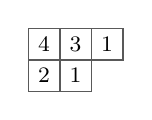
\begin{tikzpicture}[baseline={(0,-0.48)}]
\draw[gray!70!black,line width=0.5pt] (0,0) -- (0.4,0) -- (0.4,-0.4) -- (0,-0.4) -- cycle;
\draw[gray!70!black,line width=0.5pt] (0.4,0) -- (0.8,0) -- (0.8,-0.4) -- (0.4,-0.4) -- cycle;
\draw[gray!70!black,line width=0.5pt] (0.8,0) -- (1.2,0) -- (1.2,-0.4) -- (0.8,-0.4) -- cycle;
\draw[gray!70!black,line width=0.5pt] (0,-0.4) -- (0.4,-0.4) -- (0.4,-0.8) -- (0,-0.8) -- cycle;
\draw[gray!70!black,line width=0.5pt] (0.4,-0.4) -- (0.8,-0.4) -- (0.8,-0.8) -- (0.4,-0.8) -- cycle;
\node[font=\footnotesize,inner sep=0pt] at (0.2,-0.2) {$4$};
\node[font=\footnotesize,inner sep=0pt] at (0.6,-0.2) {$3$};
\node[font=\footnotesize,inner sep=0pt] at (1,-0.2) {$1$};
\node[font=\footnotesize,inner sep=0pt] at (0.2,-0.6) {$2$};
\node[font=\footnotesize,inner sep=0pt] at (0.6,-0.6) {$1$};
\end{tikzpicture}}

\newcommand{\FigMXIIIHookSquare}{%
\begin{tikzpicture}[baseline={(0,-0.48)}]
\draw[gray!70!black,line width=0.5pt] (0,0) -- (0.4,0) -- (0.4,-0.4) -- (0,-0.4) -- cycle;
\draw[gray!70!black,line width=0.5pt] (0.4,0) -- (0.8,0) -- (0.8,-0.4) -- (0.4,-0.4) -- cycle;
\draw[gray!70!black,line width=0.5pt] (0.8,0) -- (1.2,0) -- (1.2,-0.4) -- (0.8,-0.4) -- cycle;
\draw[gray!70!black,line width=0.5pt] (0,-0.4) -- (0.4,-0.4) -- (0.4,-0.8) -- (0,-0.8) -- cycle;
\draw[gray!70!black,line width=0.5pt] (0.4,-0.4) -- (0.8,-0.4) -- (0.8,-0.8) -- (0.4,-0.8) -- cycle;
\draw[gray!70!black,line width=0.5pt] (0.8,-0.4) -- (1.2,-0.4) -- (1.2,-0.8) -- (0.8,-0.8) -- cycle;
\node[font=\footnotesize,inner sep=0pt,text=cLeft] at (0.2,-0.2) {$4$};
\node[font=\footnotesize,inner sep=0pt,text=cLeft] at (0.6,-0.2) {$3$};
\node[font=\footnotesize,inner sep=0pt,text=cLeft] at (1,-0.2) {$2$};
\node[font=\footnotesize,inner sep=0pt,text=cRight] at (0.2,-0.6) {$3$};
\node[font=\footnotesize,inner sep=0pt,text=cRight] at (0.6,-0.6) {$2$};
\node[font=\footnotesize,inner sep=0pt,text=cRight] at (1,-0.6) {$1$};
\end{tikzpicture}}

\newcommand{\FigMXIIICorner}{%
\begin{tikzpicture}
\fill[cC!30] (0.72,-0.37) -- (1.08,-0.37) -- (1.08,-0.73) -- (0.72,-0.73) -- cycle;
\fill[cC!30] (0.36,-0.73) -- (0.72,-0.73) -- (0.72,-1.09) -- (0.36,-1.09) -- cycle;
\draw[gray!70!black,line width=0.5pt] (0,-0.37) -- (0.36,-0.37) -- (0.36,-0.73) -- (0,-0.73) -- cycle;
\draw[gray!70!black,line width=0.5pt] (0.36,-0.37) -- (0.72,-0.37) -- (0.72,-0.73) -- (0.36,-0.73) -- cycle;
\draw[gray!70!black,line width=0.5pt] (0.72,-0.37) -- (1.08,-0.37) -- (1.08,-0.73) -- (0.72,-0.73) -- cycle;
\draw[gray!70!black,line width=0.5pt] (0,-0.73) -- (0.36,-0.73) -- (0.36,-1.09) -- (0,-1.09) -- cycle;
\draw[gray!70!black,line width=0.5pt] (0.36,-0.73) -- (0.72,-0.73) -- (0.72,-1.09) -- (0.36,-1.09) -- cycle;
\node[font=\footnotesize] at (0.54,-1.36) {$\lambda=(3,2)$};
\node[font=\scriptsize,text=cC!80!black] at (0.54,-0.15) {角落};
\fill[cC!30] (2.72,0.3) -- (3.08,0.3) -- (3.08,-0.06) -- (2.72,-0.06) -- cycle;
\draw[gray!70!black,line width=0.5pt] (2,0.3) -- (2.36,0.3) -- (2.36,-0.06) -- (2,-0.06) -- cycle;
\draw[gray!70!black,line width=0.5pt] (2.36,0.3) -- (2.72,0.3) -- (2.72,-0.06) -- (2.36,-0.06) -- cycle;
\draw[gray!70!black,line width=0.5pt] (2.72,0.3) -- (3.08,0.3) -- (3.08,-0.06) -- (2.72,-0.06) -- cycle;
\draw[gray!70!black,line width=0.5pt] (2,-0.06) -- (2.36,-0.06) -- (2.36,-0.42) -- (2,-0.42) -- cycle;
\draw[gray!70!black,line width=0.5pt] (2.36,-0.06) -- (2.72,-0.06) -- (2.72,-0.42) -- (2.36,-0.42) -- cycle;
\node[font=\scriptsize,inner sep=0pt] at (2.18,0.12) {$1$};
\node[font=\scriptsize,inner sep=0pt] at (2.54,0.12) {$2$};
\node[font=\scriptsize,inner sep=0pt] at (2.9,0.12) {$5$};
\node[font=\scriptsize,inner sep=0pt] at (2.18,-0.24) {$3$};
\node[font=\scriptsize,inner sep=0pt] at (2.54,-0.24) {$4$};
\fill[cC!30] (4.1,0.3) -- (4.46,0.3) -- (4.46,-0.06) -- (4.1,-0.06) -- cycle;
\draw[gray!70!black,line width=0.5pt] (3.38,0.3) -- (3.74,0.3) -- (3.74,-0.06) -- (3.38,-0.06) -- cycle;
\draw[gray!70!black,line width=0.5pt] (3.74,0.3) -- (4.1,0.3) -- (4.1,-0.06) -- (3.74,-0.06) -- cycle;
\draw[gray!70!black,line width=0.5pt] (4.1,0.3) -- (4.46,0.3) -- (4.46,-0.06) -- (4.1,-0.06) -- cycle;
\draw[gray!70!black,line width=0.5pt] (3.38,-0.06) -- (3.74,-0.06) -- (3.74,-0.42) -- (3.38,-0.42) -- cycle;
\draw[gray!70!black,line width=0.5pt] (3.74,-0.06) -- (4.1,-0.06) -- (4.1,-0.42) -- (3.74,-0.42) -- cycle;
\node[font=\scriptsize,inner sep=0pt] at (3.56,0.12) {$1$};
\node[font=\scriptsize,inner sep=0pt] at (3.92,0.12) {$3$};
\node[font=\scriptsize,inner sep=0pt] at (4.28,0.12) {$5$};
\node[font=\scriptsize,inner sep=0pt] at (3.56,-0.24) {$2$};
\node[font=\scriptsize,inner sep=0pt] at (3.92,-0.24) {$4$};
\draw[-{Stealth[length=5pt]},gray!60!black,line width=0.7pt] (6.19,-0.06) -- (7.24,-0.06) node[midway,above,font=\footnotesize,text=black] {拿掉 $5$};
\draw[gray!70!black,line width=0.5pt] (7.49,0.3) -- (7.85,0.3) -- (7.85,-0.06) -- (7.49,-0.06) -- cycle;
\draw[gray!70!black,line width=0.5pt] (7.85,0.3) -- (8.21,0.3) -- (8.21,-0.06) -- (7.85,-0.06) -- cycle;
\draw[gray!70!black,line width=0.5pt] (7.49,-0.06) -- (7.85,-0.06) -- (7.85,-0.42) -- (7.49,-0.42) -- cycle;
\draw[gray!70!black,line width=0.5pt] (7.85,-0.06) -- (8.21,-0.06) -- (8.21,-0.42) -- (7.85,-0.42) -- cycle;
\node[anchor=west,font=\small] at (8.51,-0.06) {$f^{(2,2)}=2$};
\fill[cC!30] (2.36,-1.41) -- (2.72,-1.41) -- (2.72,-1.77) -- (2.36,-1.77) -- cycle;
\draw[gray!70!black,line width=0.5pt] (2,-1.05) -- (2.36,-1.05) -- (2.36,-1.41) -- (2,-1.41) -- cycle;
\draw[gray!70!black,line width=0.5pt] (2.36,-1.05) -- (2.72,-1.05) -- (2.72,-1.41) -- (2.36,-1.41) -- cycle;
\draw[gray!70!black,line width=0.5pt] (2.72,-1.05) -- (3.08,-1.05) -- (3.08,-1.41) -- (2.72,-1.41) -- cycle;
\draw[gray!70!black,line width=0.5pt] (2,-1.41) -- (2.36,-1.41) -- (2.36,-1.77) -- (2,-1.77) -- cycle;
\draw[gray!70!black,line width=0.5pt] (2.36,-1.41) -- (2.72,-1.41) -- (2.72,-1.77) -- (2.36,-1.77) -- cycle;
\node[font=\scriptsize,inner sep=0pt] at (2.18,-1.23) {$1$};
\node[font=\scriptsize,inner sep=0pt] at (2.54,-1.23) {$2$};
\node[font=\scriptsize,inner sep=0pt] at (2.9,-1.23) {$3$};
\node[font=\scriptsize,inner sep=0pt] at (2.18,-1.59) {$4$};
\node[font=\scriptsize,inner sep=0pt] at (2.54,-1.59) {$5$};
\fill[cC!30] (3.74,-1.41) -- (4.1,-1.41) -- (4.1,-1.77) -- (3.74,-1.77) -- cycle;
\draw[gray!70!black,line width=0.5pt] (3.38,-1.05) -- (3.74,-1.05) -- (3.74,-1.41) -- (3.38,-1.41) -- cycle;
\draw[gray!70!black,line width=0.5pt] (3.74,-1.05) -- (4.1,-1.05) -- (4.1,-1.41) -- (3.74,-1.41) -- cycle;
\draw[gray!70!black,line width=0.5pt] (4.1,-1.05) -- (4.46,-1.05) -- (4.46,-1.41) -- (4.1,-1.41) -- cycle;
\draw[gray!70!black,line width=0.5pt] (3.38,-1.41) -- (3.74,-1.41) -- (3.74,-1.77) -- (3.38,-1.77) -- cycle;
\draw[gray!70!black,line width=0.5pt] (3.74,-1.41) -- (4.1,-1.41) -- (4.1,-1.77) -- (3.74,-1.77) -- cycle;
\node[font=\scriptsize,inner sep=0pt] at (3.56,-1.23) {$1$};
\node[font=\scriptsize,inner sep=0pt] at (3.92,-1.23) {$2$};
\node[font=\scriptsize,inner sep=0pt] at (4.28,-1.23) {$4$};
\node[font=\scriptsize,inner sep=0pt] at (3.56,-1.59) {$3$};
\node[font=\scriptsize,inner sep=0pt] at (3.92,-1.59) {$5$};
\fill[cC!30] (5.12,-1.41) -- (5.48,-1.41) -- (5.48,-1.77) -- (5.12,-1.77) -- cycle;
\draw[gray!70!black,line width=0.5pt] (4.76,-1.05) -- (5.12,-1.05) -- (5.12,-1.41) -- (4.76,-1.41) -- cycle;
\draw[gray!70!black,line width=0.5pt] (5.12,-1.05) -- (5.48,-1.05) -- (5.48,-1.41) -- (5.12,-1.41) -- cycle;
\draw[gray!70!black,line width=0.5pt] (5.48,-1.05) -- (5.84,-1.05) -- (5.84,-1.41) -- (5.48,-1.41) -- cycle;
\draw[gray!70!black,line width=0.5pt] (4.76,-1.41) -- (5.12,-1.41) -- (5.12,-1.77) -- (4.76,-1.77) -- cycle;
\draw[gray!70!black,line width=0.5pt] (5.12,-1.41) -- (5.48,-1.41) -- (5.48,-1.77) -- (5.12,-1.77) -- cycle;
\node[font=\scriptsize,inner sep=0pt] at (4.94,-1.23) {$1$};
\node[font=\scriptsize,inner sep=0pt] at (5.3,-1.23) {$3$};
\node[font=\scriptsize,inner sep=0pt] at (5.66,-1.23) {$4$};
\node[font=\scriptsize,inner sep=0pt] at (4.94,-1.59) {$2$};
\node[font=\scriptsize,inner sep=0pt] at (5.3,-1.59) {$5$};
\draw[-{Stealth[length=5pt]},gray!60!black,line width=0.7pt] (6.19,-1.41) -- (7.24,-1.41) node[midway,above,font=\footnotesize,text=black] {拿掉 $5$};
\draw[gray!70!black,line width=0.5pt] (7.49,-1.05) -- (7.85,-1.05) -- (7.85,-1.41) -- (7.49,-1.41) -- cycle;
\draw[gray!70!black,line width=0.5pt] (7.85,-1.05) -- (8.21,-1.05) -- (8.21,-1.41) -- (7.85,-1.41) -- cycle;
\draw[gray!70!black,line width=0.5pt] (8.21,-1.05) -- (8.57,-1.05) -- (8.57,-1.41) -- (8.21,-1.41) -- cycle;
\draw[gray!70!black,line width=0.5pt] (7.49,-1.41) -- (7.85,-1.41) -- (7.85,-1.77) -- (7.49,-1.77) -- cycle;
\node[anchor=west,font=\small] at (8.87,-1.41) {$f^{(3,1)}=3$};
\end{tikzpicture}}

\newcommand{\FigMXIVWalks}{%
\begin{tikzpicture}
\fill[cC!30] (1.24,-0.62) -- (1.86,-0.62) -- (1.86,-1.24) -- (1.24,-1.24) -- cycle;
\draw[gray!70!black,line width=0.5pt] (0,0) -- (0.62,0) -- (0.62,-0.62) -- (0,-0.62) -- cycle;
\draw[gray!70!black,line width=0.5pt] (0.62,0) -- (1.24,0) -- (1.24,-0.62) -- (0.62,-0.62) -- cycle;
\draw[gray!70!black,line width=0.5pt] (1.24,0) -- (1.86,0) -- (1.86,-0.62) -- (1.24,-0.62) -- cycle;
\draw[gray!70!black,line width=0.5pt] (1.86,0) -- (2.48,0) -- (2.48,-0.62) -- (1.86,-0.62) -- cycle;
\draw[gray!70!black,line width=0.5pt] (0,-0.62) -- (0.62,-0.62) -- (0.62,-1.24) -- (0,-1.24) -- cycle;
\draw[gray!70!black,line width=0.5pt] (0.62,-0.62) -- (1.24,-0.62) -- (1.24,-1.24) -- (0.62,-1.24) -- cycle;
\draw[gray!70!black,line width=0.5pt] (1.24,-0.62) -- (1.86,-0.62) -- (1.86,-1.24) -- (1.24,-1.24) -- cycle;
\draw[gray!70!black,line width=0.5pt] (0,-1.24) -- (0.62,-1.24) -- (0.62,-1.86) -- (0,-1.86) -- cycle;
\node[font=\footnotesize,inner sep=0pt,text=gray!55!black] at (0.31,-0.31) {$6$};
\node[font=\footnotesize,inner sep=0pt,text=gray!55!black] at (0.93,-0.31) {$4$};
\node[font=\footnotesize,inner sep=0pt,text=gray!55!black] at (1.55,-0.31) {$3$};
\node[font=\footnotesize,inner sep=0pt,text=gray!55!black] at (2.17,-0.31) {$1$};
\node[font=\footnotesize,inner sep=0pt,text=gray!55!black] at (0.31,-0.93) {$4$};
\node[font=\footnotesize,inner sep=0pt,text=gray!55!black] at (0.93,-0.93) {$2$};
\node[font=\footnotesize,inner sep=0pt,text=gray!55!black] at (1.55,-0.93) {$1$};
\node[font=\footnotesize,inner sep=0pt,text=gray!55!black] at (0.31,-1.55) {$1$};
\draw[cTop,line width=1.4pt] (0.07,-0.07) rectangle (0.55,-0.55);
\draw[-{Stealth[length=4.5pt,width=4pt]},cTop,line width=1.1pt,shorten <=1pt,shorten >=1pt] (0.31,-0.136) to[bend left=45] (1.55,-0.136);
\draw[-{Stealth[length=4.5pt,width=4pt]},cTop,line width=1.1pt,shorten <=1pt,shorten >=1pt] (1.376,-0.31) to[bend right=45] (1.376,-0.93);
\node[font=\scriptsize\bfseries,text=cLeft] at (-0.32,-0.31) {1};
\node[font=\scriptsize\bfseries,text=cLeft] at (-0.32,-0.93) {2};
\node[font=\scriptsize,text=gray!60!black] at (-0.32,-1.55) {3};
\node[font=\scriptsize\bfseries,text=cRight] at (0.31,0.2) {1};
\node[font=\scriptsize,text=gray!60!black] at (0.93,0.2) {2};
\node[font=\scriptsize\bfseries,text=cRight] at (1.55,0.2) {3};
\node[font=\scriptsize,text=gray!60!black] at (2.17,0.2) {4};
\node[font=\small] at (1.24,-2.31) {$\frac{1}{8}\cdot\frac{1}{5}\cdot\frac{1}{2}=\frac{1}{80}$};
\node[font=\small] at (1.24,-2.86) {$\textcolor{cLeft}{A=\{1,2\}},\ \textcolor{cRight}{B=\{1,3\}}$};
\fill[cC!30] (6.64,-0.62) -- (7.26,-0.62) -- (7.26,-1.24) -- (6.64,-1.24) -- cycle;
\draw[gray!70!black,line width=0.5pt] (5.4,0) -- (6.02,0) -- (6.02,-0.62) -- (5.4,-0.62) -- cycle;
\draw[gray!70!black,line width=0.5pt] (6.02,0) -- (6.64,0) -- (6.64,-0.62) -- (6.02,-0.62) -- cycle;
\draw[gray!70!black,line width=0.5pt] (6.64,0) -- (7.26,0) -- (7.26,-0.62) -- (6.64,-0.62) -- cycle;
\draw[gray!70!black,line width=0.5pt] (7.26,0) -- (7.88,0) -- (7.88,-0.62) -- (7.26,-0.62) -- cycle;
\draw[gray!70!black,line width=0.5pt] (5.4,-0.62) -- (6.02,-0.62) -- (6.02,-1.24) -- (5.4,-1.24) -- cycle;
\draw[gray!70!black,line width=0.5pt] (6.02,-0.62) -- (6.64,-0.62) -- (6.64,-1.24) -- (6.02,-1.24) -- cycle;
\draw[gray!70!black,line width=0.5pt] (6.64,-0.62) -- (7.26,-0.62) -- (7.26,-1.24) -- (6.64,-1.24) -- cycle;
\draw[gray!70!black,line width=0.5pt] (5.4,-1.24) -- (6.02,-1.24) -- (6.02,-1.86) -- (5.4,-1.86) -- cycle;
\node[font=\footnotesize,inner sep=0pt,text=gray!55!black] at (5.71,-0.31) {$6$};
\node[font=\footnotesize,inner sep=0pt,text=gray!55!black] at (6.33,-0.31) {$4$};
\node[font=\footnotesize,inner sep=0pt,text=gray!55!black] at (6.95,-0.31) {$3$};
\node[font=\footnotesize,inner sep=0pt,text=gray!55!black] at (7.57,-0.31) {$1$};
\node[font=\footnotesize,inner sep=0pt,text=gray!55!black] at (5.71,-0.93) {$4$};
\node[font=\footnotesize,inner sep=0pt,text=gray!55!black] at (6.33,-0.93) {$2$};
\node[font=\footnotesize,inner sep=0pt,text=gray!55!black] at (6.95,-0.93) {$1$};
\node[font=\footnotesize,inner sep=0pt,text=gray!55!black] at (5.71,-1.55) {$1$};
\draw[cTop,line width=1.4pt] (5.47,-0.07) rectangle (5.95,-0.55);
\draw[-{Stealth[length=4.5pt,width=4pt]},cTop,line width=1.1pt,shorten <=1pt,shorten >=1pt] (5.536,-0.31) to[bend right=45] (5.536,-0.93);
\draw[-{Stealth[length=4.5pt,width=4pt]},cTop,line width=1.1pt,shorten <=1pt,shorten >=1pt] (5.71,-0.756) to[bend left=45] (6.95,-0.756);
\node[font=\scriptsize\bfseries,text=cLeft] at (5.08,-0.31) {1};
\node[font=\scriptsize\bfseries,text=cLeft] at (5.08,-0.93) {2};
\node[font=\scriptsize,text=gray!60!black] at (5.08,-1.55) {3};
\node[font=\scriptsize\bfseries,text=cRight] at (5.71,0.2) {1};
\node[font=\scriptsize,text=gray!60!black] at (6.33,0.2) {2};
\node[font=\scriptsize\bfseries,text=cRight] at (6.95,0.2) {3};
\node[font=\scriptsize,text=gray!60!black] at (7.57,0.2) {4};
\node[font=\small] at (6.64,-2.31) {$\frac{1}{8}\cdot\frac{1}{5}\cdot\frac{1}{3}=\frac{1}{120}$};
\node[font=\small] at (6.64,-2.86) {$\textcolor{cLeft}{A=\{1,2\}},\ \textcolor{cRight}{B=\{1,3\}}$};
\end{tikzpicture}}

\newcommand{\FigMXIVIdentity}{%
\begin{tikzpicture}
\fill[yellow!55] (0.42,0) -- (0.84,0) -- (0.84,-0.42) -- (0.42,-0.42) -- cycle;
\fill[yellow!55] (0.84,0) -- (1.26,0) -- (1.26,-0.42) -- (0.84,-0.42) -- cycle;
\fill[yellow!55] (1.26,0) -- (1.68,0) -- (1.68,-0.42) -- (1.26,-0.42) -- cycle;
\fill[yellow!55] (0,-0.42) -- (0.42,-0.42) -- (0.42,-0.84) -- (0,-0.84) -- cycle;
\fill[yellow!55] (0,-0.84) -- (0.42,-0.84) -- (0.42,-1.26) -- (0,-1.26) -- cycle;
\draw[gray!70!black,line width=0.5pt] (0,0) -- (0.42,0) -- (0.42,-0.42) -- (0,-0.42) -- cycle;
\draw[gray!70!black,line width=0.5pt] (0.42,0) -- (0.84,0) -- (0.84,-0.42) -- (0.42,-0.42) -- cycle;
\draw[gray!70!black,line width=0.5pt] (0.84,0) -- (1.26,0) -- (1.26,-0.42) -- (0.84,-0.42) -- cycle;
\draw[gray!70!black,line width=0.5pt] (1.26,0) -- (1.68,0) -- (1.68,-0.42) -- (1.26,-0.42) -- cycle;
\draw[gray!70!black,line width=0.5pt] (0,-0.42) -- (0.42,-0.42) -- (0.42,-0.84) -- (0,-0.84) -- cycle;
\draw[gray!70!black,line width=0.5pt] (0.42,-0.42) -- (0.84,-0.42) -- (0.84,-0.84) -- (0.42,-0.84) -- cycle;
\draw[gray!70!black,line width=0.5pt] (0.84,-0.42) -- (1.26,-0.42) -- (1.26,-0.84) -- (0.84,-0.84) -- cycle;
\draw[gray!70!black,line width=0.5pt] (0,-0.84) -- (0.42,-0.84) -- (0.42,-1.26) -- (0,-1.26) -- cycle;
\draw[cTop,line width=1.3pt] (0.06,-0.06) rectangle (0.36,-0.36);
\draw[cC,line width=1.3pt,densely dashed] (0.9,-0.48) rectangle (1.2,-0.78);
\node[font=\small] at (0.84,0.32) {$h(a,b)-1$};
\node[font=\normalsize] at (0.84,-1.58) {$5$};
\fill[cLeft!35] (4.01,0) -- (4.43,0) -- (4.43,-0.42) -- (4.01,-0.42) -- cycle;
\fill[cLeft!35] (3.59,-0.42) -- (4.01,-0.42) -- (4.01,-0.84) -- (3.59,-0.84) -- cycle;
\draw[gray!70!black,line width=0.5pt] (2.75,0) -- (3.17,0) -- (3.17,-0.42) -- (2.75,-0.42) -- cycle;
\draw[gray!70!black,line width=0.5pt] (3.17,0) -- (3.59,0) -- (3.59,-0.42) -- (3.17,-0.42) -- cycle;
\draw[gray!70!black,line width=0.5pt] (3.59,0) -- (4.01,0) -- (4.01,-0.42) -- (3.59,-0.42) -- cycle;
\draw[gray!70!black,line width=0.5pt] (4.01,0) -- (4.43,0) -- (4.43,-0.42) -- (4.01,-0.42) -- cycle;
\draw[gray!70!black,line width=0.5pt] (2.75,-0.42) -- (3.17,-0.42) -- (3.17,-0.84) -- (2.75,-0.84) -- cycle;
\draw[gray!70!black,line width=0.5pt] (3.17,-0.42) -- (3.59,-0.42) -- (3.59,-0.84) -- (3.17,-0.84) -- cycle;
\draw[gray!70!black,line width=0.5pt] (3.59,-0.42) -- (4.01,-0.42) -- (4.01,-0.84) -- (3.59,-0.84) -- cycle;
\draw[gray!70!black,line width=0.5pt] (2.75,-0.84) -- (3.17,-0.84) -- (3.17,-1.26) -- (2.75,-1.26) -- cycle;
\draw[cTop,line width=1.3pt] (3.65,-0.06) rectangle (3.95,-0.36);
\draw[cC,line width=1.3pt,densely dashed] (3.65,-0.48) rectangle (3.95,-0.78);
\node[font=\small] at (3.59,0.32) {$h(a,\beta)-1$};
\node[font=\normalsize] at (3.59,-1.58) {$2$};
\fill[cRight!30] (5.92,-0.42) -- (6.34,-0.42) -- (6.34,-0.84) -- (5.92,-0.84) -- cycle;
\fill[cRight!30] (6.34,-0.42) -- (6.76,-0.42) -- (6.76,-0.84) -- (6.34,-0.84) -- cycle;
\fill[cRight!30] (5.5,-0.84) -- (5.92,-0.84) -- (5.92,-1.26) -- (5.5,-1.26) -- cycle;
\draw[gray!70!black,line width=0.5pt] (5.5,0) -- (5.92,0) -- (5.92,-0.42) -- (5.5,-0.42) -- cycle;
\draw[gray!70!black,line width=0.5pt] (5.92,0) -- (6.34,0) -- (6.34,-0.42) -- (5.92,-0.42) -- cycle;
\draw[gray!70!black,line width=0.5pt] (6.34,0) -- (6.76,0) -- (6.76,-0.42) -- (6.34,-0.42) -- cycle;
\draw[gray!70!black,line width=0.5pt] (6.76,0) -- (7.18,0) -- (7.18,-0.42) -- (6.76,-0.42) -- cycle;
\draw[gray!70!black,line width=0.5pt] (5.5,-0.42) -- (5.92,-0.42) -- (5.92,-0.84) -- (5.5,-0.84) -- cycle;
\draw[gray!70!black,line width=0.5pt] (5.92,-0.42) -- (6.34,-0.42) -- (6.34,-0.84) -- (5.92,-0.84) -- cycle;
\draw[gray!70!black,line width=0.5pt] (6.34,-0.42) -- (6.76,-0.42) -- (6.76,-0.84) -- (6.34,-0.84) -- cycle;
\draw[gray!70!black,line width=0.5pt] (5.5,-0.84) -- (5.92,-0.84) -- (5.92,-1.26) -- (5.5,-1.26) -- cycle;
\draw[cTop,line width=1.3pt] (5.56,-0.48) rectangle (5.86,-0.78);
\draw[cC,line width=1.3pt,densely dashed] (6.4,-0.48) rectangle (6.7,-0.78);
\node[font=\small] at (6.34,0.32) {$h(\alpha,b)-1$};
\node[font=\normalsize] at (6.34,-1.58) {$3$};
\node[font=\large] at (2.215,-0.63) {$=$};
\node[font=\large] at (4.965,-0.63) {$+$};
\end{tikzpicture}}

\newcommand{\FigMXIVRemove}{%
\begin{tikzpicture}
\fill[cLeft!30] (1.1,0) -- (1.65,0) -- (1.65,-0.55) -- (1.1,-0.55) -- cycle;
\fill[cRight!28] (0,-0.55) -- (0.55,-0.55) -- (0.55,-1.1) -- (0,-1.1) -- cycle;
\fill[cRight!28] (0.55,-0.55) -- (1.1,-0.55) -- (1.1,-1.1) -- (0.55,-1.1) -- cycle;
\fill[cC!30] (1.1,-0.55) -- (1.65,-0.55) -- (1.65,-1.1) -- (1.1,-1.1) -- cycle;
\draw[gray!70!black,line width=0.5pt] (0,0) -- (0.55,0) -- (0.55,-0.55) -- (0,-0.55) -- cycle;
\draw[gray!70!black,line width=0.5pt] (0.55,0) -- (1.1,0) -- (1.1,-0.55) -- (0.55,-0.55) -- cycle;
\draw[gray!70!black,line width=0.5pt] (1.1,0) -- (1.65,0) -- (1.65,-0.55) -- (1.1,-0.55) -- cycle;
\draw[gray!70!black,line width=0.5pt] (1.65,0) -- (2.2,0) -- (2.2,-0.55) -- (1.65,-0.55) -- cycle;
\draw[gray!70!black,line width=0.5pt] (0,-0.55) -- (0.55,-0.55) -- (0.55,-1.1) -- (0,-1.1) -- cycle;
\draw[gray!70!black,line width=0.5pt] (0.55,-0.55) -- (1.1,-0.55) -- (1.1,-1.1) -- (0.55,-1.1) -- cycle;
\draw[gray!70!black,line width=0.5pt] (1.1,-0.55) -- (1.65,-0.55) -- (1.65,-1.1) -- (1.1,-1.1) -- cycle;
\draw[gray!70!black,line width=0.5pt] (0,-1.1) -- (0.55,-1.1) -- (0.55,-1.65) -- (0,-1.65) -- cycle;
\node[font=\small,inner sep=0pt] at (0.275,-0.275) {$6$};
\node[font=\small,inner sep=0pt] at (0.825,-0.275) {$4$};
\node[font=\small,inner sep=0pt] at (1.375,-0.275) {$3$};
\node[font=\small,inner sep=0pt] at (1.925,-0.275) {$1$};
\node[font=\small,inner sep=0pt] at (0.275,-0.825) {$4$};
\node[font=\small,inner sep=0pt] at (0.825,-0.825) {$2$};
\node[font=\small,inner sep=0pt] at (1.375,-0.825) {$1$};
\node[font=\small,inner sep=0pt] at (0.275,-1.375) {$1$};
\fill[cLeft!30] (5.3,0) -- (5.85,0) -- (5.85,-0.55) -- (5.3,-0.55) -- cycle;
\fill[cRight!28] (4.2,-0.55) -- (4.75,-0.55) -- (4.75,-1.1) -- (4.2,-1.1) -- cycle;
\fill[cRight!28] (4.75,-0.55) -- (5.3,-0.55) -- (5.3,-1.1) -- (4.75,-1.1) -- cycle;
\draw[gray!70!black,line width=0.5pt] (4.2,0) -- (4.75,0) -- (4.75,-0.55) -- (4.2,-0.55) -- cycle;
\draw[gray!70!black,line width=0.5pt] (4.75,0) -- (5.3,0) -- (5.3,-0.55) -- (4.75,-0.55) -- cycle;
\draw[gray!70!black,line width=0.5pt] (5.3,0) -- (5.85,0) -- (5.85,-0.55) -- (5.3,-0.55) -- cycle;
\draw[gray!70!black,line width=0.5pt] (5.85,0) -- (6.4,0) -- (6.4,-0.55) -- (5.85,-0.55) -- cycle;
\draw[gray!70!black,line width=0.5pt] (4.2,-0.55) -- (4.75,-0.55) -- (4.75,-1.1) -- (4.2,-1.1) -- cycle;
\draw[gray!70!black,line width=0.5pt] (4.75,-0.55) -- (5.3,-0.55) -- (5.3,-1.1) -- (4.75,-1.1) -- cycle;
\draw[gray!70!black,line width=0.5pt] (4.2,-1.1) -- (4.75,-1.1) -- (4.75,-1.65) -- (4.2,-1.65) -- cycle;
\node[font=\small,inner sep=0pt] at (4.475,-0.275) {$6$};
\node[font=\small,inner sep=0pt] at (5.025,-0.275) {$4$};
\node[font=\small,inner sep=0pt] at (5.575,-0.275) {$2$};
\node[font=\small,inner sep=0pt] at (6.125,-0.275) {$1$};
\node[font=\small,inner sep=0pt] at (4.475,-0.825) {$3$};
\node[font=\small,inner sep=0pt] at (5.025,-0.825) {$1$};
\node[font=\small,inner sep=0pt] at (4.475,-1.375) {$1$};
\draw[gray!60,densely dashed,line width=0.6pt] (5.3,-0.55) rectangle (5.85,-1.1);
\draw[-{Stealth[length=5pt]},gray!60!black,line width=0.7pt] (2.55,-0.825) -- (3.85,-0.825) node[midway,above,font=\footnotesize,text=black] {拿掉 $c$};
\node[font=\small] at (1.1,0.3) {$\lambda=(4,3,1)$};
\node[font=\small] at (1.1,-1.95) {$H(\lambda)=576$};
\node[font=\small] at (5.3,0.3) {$\lambda-c=(4,2,1)$};
\node[font=\small] at (5.3,-1.95) {$H(\lambda-c)=144$};
\end{tikzpicture}}


% ---------------------------------------------------------------------
\subsection{標準 Young 表與 Dyck 路徑}\label{sec:m12}

這一節看兩列等長的形狀 $(n,n)$：它的標準 Young 表就是 Dyck 路徑 \mitref{L4}。
回憶第~\ref{sec:m11} 節的\textbf{標準 Young 表}：把 $1,2,\ldots,|\lambda|$（$|\lambda|$ 是格子數）各填一次到形狀 $\lambda$ 的 Young 圖，
每一列由左到右、每一行由上到下都遞增；個數記為 $f^{\lambda}$。

\textbf{讀表的規則。}依序讀 $1,2,\ldots,2n$：數字 $i$ 在第一列，第 $i$ 步就往上（U）；
在第二列，第 $i$ 步就往下（D）。貫穿的例子：第一列是 $1,2,4$、第二列是 $3,5,6$，
所以第 1、2、4 步是 U，第 3、5、6 步是 D，得到 UUDUDD（圖~\ref{fig:m12-convert}）。

\begin{figure}[H]
\centering
\FigMXIIConvert
\caption{形狀 $(3,3)$ 的表：\textcolor{cLeft}{第一列的數 $\to$ U}、\textcolor{cRight}{第二列的數 $\to$ D}。
例子 $\begin{smallmatrix}1&2&4\\3&5&6\end{smallmatrix}$ 變成 Dyck 路徑 UUDUDD。}
\label{fig:m12-convert}
\end{figure}

\textbf{為什麼不會掉到地面以下。}記 $T_{r,j}$ 為第 $r$ 列第 $j$ 格的數。
列是遞增的，所以第 $j$ 個 U 是第 $T_{1,j}$ 步，第 $j$ 個 D 是第 $T_{2,j}$ 步。
行也是遞增的：$T_{1,j}<T_{2,j}$，也就是\textbf{第 $j$ 個 D 之前，一定已經有第 $j$ 個 U}。
所以任何時候 U 的個數都 $\ge$ D 的個數，路徑不低於地面。例子的三行是 $1<3$、$2<5$、$4<6$。

\textbf{反過來。}給一條半長 $n$ 的 Dyck 路徑，把 U 所在的步號由小到大填進第一列、D 所在的步號填進第二列。
兩列自動遞增；路徑不低於地面，表示第 $j$ 個 U 比第 $j$ 個 D 早，也就是每一行遞增。
兩個方向互為反函數，所以是一一對應。

\begin{thmbox}[兩列的標準 Young 表]
形狀 $(n,n)$ 的標準 Young 表與半長 $n$ 的 Dyck 路徑一一對應，所以 $f^{(n,n)}=C_n$。
\end{thmbox}

\begin{figure}[H]
\centering
\FigMXIIAll
\caption{形狀 $(3,3)$ 的 5 個標準 Young 表與對應的 5 條 Dyck 路徑（順序同動畫 M12），
\textcolor{cTop}{虛線框}是貫穿的例子。}
\label{fig:m12-all}
\end{figure}

程式逐一列舉 $n=1,\ldots,6$：$f^{(n,n)}=1,2,5,14,42,132$，與 $C_n$ 相同。
換成投票問題的語言（圖~\ref{fig:ballot}）：第 $i$ 張票投給 A 就把 $i$ 放進第一列、投給 B 就放進第二列，
「行遞增」就是「A 從不落後」；例子對應開票順序 AABABB。

\textbf{一般的形狀。}$\lambda=(\lambda_1,\ldots,\lambda_k)$ 有 $k$ 列。
數字 $i$ 在第 $r$ 列，第 $i$ 步就走 $e_r$（第 $r$ 個座標加 1）。
讀完前 $t$ 個數之後的位置 $(x_1,\ldots,x_k)$，就是各列已經填了幾格。
第 $r$ 列要填第 $j$ 格時，它上面那格（第 $r-1$ 列第 $j$ 格）必須早就填好，也就是填完之後仍有 $x_{r-1}\ge x_r$。
所以「每一行遞增」等於\textbf{一路上都保持 $x_1\ge x_2\ge\cdots\ge x_k$}（表~\ref{tab:m12-general}）。

\begin{thmbox}[標準 Young 表 $=$ 格子路徑]
形狀 $\lambda$ 的標準 Young 表，一一對應到 $\mathbb{Z}^k$ 中從原點走到 $\lambda$、每一步是某個 $e_r$、
一路保持 $x_1\ge x_2\ge\cdots\ge x_k$ 的格子路徑。
$\lambda=(n,n)$ 時，$x_1\ge x_2$ 就是「U 不比 D 少」，回到 Dyck 路徑。
\end{thmbox}

\begin{table}[H]
\centering
\small
\renewcommand{\arraystretch}{1.15}
\begin{tabular}{@{}c@{\qquad}cccccl@{}}
\toprule
表 & 讀完 1 & 讀完 2 & 讀完 3 & 讀完 4 & 讀完 5 & \\
\midrule
\FigMXIIGenGood & $(1,0,0)$ & $(1,1,0)$ & $(2,1,0)$ & $(2,1,1)$ & $(2,2,1)$ & 一路 $x_1\ge x_2\ge x_3$ \\[0.5em]
\FigMXIIGenBad & $(1,0,0)$ & $(1,1,0)$ & $(1,1,1)$ & $\textcolor{cBad}{(1,2,1)}$ & $(2,2,1)$
  & \textcolor{cBad}{$x_2>x_1$，不是標準 Young 表}\\
\bottomrule
\end{tabular}
\caption{形狀 $\lambda=(2,2,1)$。上：依序走 $e_1,e_2,e_1,e_3,e_2$，每一步都有 $x_1\ge x_2\ge x_3$，終點是 $\lambda$。
下：把 5 放在 4 上面（\textcolor{cBad}{紅框}那一行 $5>4$），讀到 4 時 $x_2=2>x_1=1$，路徑跑出區域。}
\label{tab:m12-general}
\end{table}

% ---------------------------------------------------------------------
\subsection{鉤長公式}\label{sec:m13}

$f^{\lambda}$ 有一條漂亮的公式，只用到每一格的「鉤長」\mitref{L4}。

\textbf{鉤。}格子 $c$ 的\textbf{鉤}（hook）由三部分組成：$c$ 自己、同一列在它右邊的格子（\textbf{臂}，arm）、
同一行在它下面的格子（\textbf{腿}，leg）。鉤裡的格子數叫做\textbf{鉤長}：
\[
h(c)=\operatorname{arm}(c)+\operatorname{leg}(c)+1 .
\]
$c$ 在第 $i$ 列第 $j$ 行時，$\operatorname{arm}(c)=\lambda_i-j$、$\operatorname{leg}(c)=\lambda'_j-i$，
其中 $\lambda'_j$ 是第 $j$ 行的長度。例：$\lambda=(4,3,1)$ 的格子 $c=(1,2)$ 有 2 格臂、1 格腿，
$h(c)=4$（圖~\ref{fig:m13-hook} 左）。

\begin{figure}[H]
\centering
\FigMXIIIHook
\caption{$\lambda=(4,3,1)$。左：格子 $c=(1,2)$ 的鉤，由\textcolor{cTop}{橘色的 $c$ 自己}和黃色的臂、腿組成。右：每一格的鉤長。}
\label{fig:m13-hook}
\end{figure}

把每一格的鉤長乘起來：
\[
H(\lambda)=\prod_{c\in\lambda}h(c)=6\cdot4\cdot3\cdot1\cdot4\cdot2\cdot1\cdot1=576,\qquad
\frac{8!}{H(\lambda)}=\frac{40320}{576}=70 .
\]
而形狀 $(4,3,1)$ 的標準 Young 表恰有 70 個（程式列舉）。這不是巧合：

\begin{thmbox}[鉤長公式（Frame--Robinson--Thrall，1954）]
$\lambda$ 是 $n$ 的分割時，形狀 $\lambda$ 的標準 Young 表個數是
\begin{equation}\label{eq:m13-hook}
f^{\lambda}=\frac{n!}{\prod_{c\in\lambda}h(c)}=\frac{n!}{H(\lambda)} .
\end{equation}
\end{thmbox}

\textbf{驗算。}第~\ref{sec:m11} 節列出的 $(3,2)$，以及上一節的 $(3,3)$（格子裡是鉤長）：
\[
\FigMXIIIHookSmall\quad \frac{5!}{4\cdot3\cdot1\cdot2\cdot1}=\frac{120}{24}=5,
\qquad\qquad
\FigMXIIIHookSquare\quad \frac{6!}{(4\cdot3\cdot2)(3\cdot2\cdot1)}=\frac{720}{144}=5=C_3 .
\]
一般的 $(n,n)$：第一列的鉤長是 \textcolor{cLeft}{$n+1,n,\ldots,2$}，第二列是 \textcolor{cRight}{$n,n-1,\ldots,1$}，
所以 $H=(n+1)!\,n!$，
\[
f^{(n,n)}=\frac{(2n)!}{(n+1)!\,n!}=C_n ,
\]
這是 $f^{(n,n)}=C_n$ 的第二個證明。

\textbf{角落遞迴。}以下 $\lambda$ 是 $n$ 的分割。右邊和下面都沒有格子的格子叫\textbf{角落}；拿掉角落 $c$，剩下的 $\lambda-c$ 仍是 Young 圖。
在標準 Young 表裡，最大的數 $n$ 一定在某個角落：它右邊或下面的數都要比 $n$ 大，所以那裡不能有格子。
拿掉 $n$，剩下的是形狀 $\lambda-c$ 的標準 Young 表；反過來，在 $\lambda-c$ 的表的格子 $c$ 填上 $n$，
就得到 $\lambda$ 的表。所以
\begin{equation}\label{eq:m13-corner}
f^{\lambda}=\sum_{c\ \text{是角落}}f^{\lambda-c},\qquad f^{\varnothing}=1 .
\end{equation}
例：$(3,2)$ 的 5 個表依 5 的位置分成 $2+3$ 個（圖~\ref{fig:m13-corner}），
$f^{(3,2)}=f^{(2,2)}+f^{(3,1)}=2+3=5$。

\begin{figure}[H]
\centering
\FigMXIIICorner
\caption{角落遞迴：$(3,2)$ 的 5 個表依最大數 5 所在的\textcolor{cC}{角落}分成兩組，拿掉 5 就是較小形狀的表。}
\label{fig:m13-corner}
\end{figure}

\textbf{化約成「機率和為 1」。}令 $F(\lambda)=n!/H(\lambda)$。要證 $F=f$，對 $n$ 歸納：
$F(\varnothing)=1$，所以只要再證明 $F$ 也滿足角落遞迴 \eqref{eq:m13-corner}。
設 $n-1$ 格的形狀都已有 $f=F$，則 $f^{\lambda}=\sum_c F(\lambda-c)$，只需證 $\sum_c F(\lambda-c)=F(\lambda)$。
兩邊除以 $F(\lambda)$：
\begin{equation}\label{eq:m13-reduce}
\sum_{c}\frac{(n-1)!}{H(\lambda-c)}\cdot\frac{H(\lambda)}{n!}
=\sum_{c\ \text{是角落}}\frac{1}{n}\cdot\frac{H(\lambda)}{H(\lambda-c)}=1 .
\end{equation}
驗算 $(3,2)$：$H(3,2)=24$、$H(2,2)=12$、$H(3,1)=8$，
\[
\frac15\cdot\frac{24}{12}+\frac15\cdot\frac{24}{8}=\frac25+\frac35=1 .
\]
式 \eqref{eq:m13-reduce} 的每一項都是正的、加起來是 1，很像機率。
下一節的「鉤上漫步」讓它們真的變成機率：停在角落 $c$ 的機率。

% ---------------------------------------------------------------------
\subsection{鉤上漫步的證明}\label{sec:m14}

這一節用 Greene、Nijenhuis 與 Wilf（1979）的機率論證 \mitref{L4} 證明式 \eqref{eq:m13-reduce}，
於是得到鉤長公式。例子沿用 $\lambda=(4,3,1)$，$n=8$。格子 $(i,j)$ 指第 $i$ 列第 $j$ 行。

\textbf{(1) 鉤上漫步。}
\begin{enumerate}[leftmargin=1.6em]
  \item 從 $n$ 格中\textbf{均勻}隨機選一格當起點，每格機率 $\frac1n$。
  \item 在格子 $x$ 上，若 $h(x)>1$，就從 $x$ 的鉤上「$x$ 以外的 $h(x)-1$ 格」均勻選一格跳過去，
        每格機率 $\frac{1}{h(x)-1}$。
  \item $h(x)=1$ 時停止。
\end{enumerate}
每一跳都往右或往下，所以一定會停。$h(x)=1$ 表示右邊、下面都沒有格子，也就是角落：
\textbf{漫步一定停在某個角落}。圖~\ref{fig:m14-walks} 左是一次漫步：從 $(1,1)$（$h=6$）以機率 $\frac15$ 跳到 $(1,3)$（$h=3$），
再以 $\frac12$ 跳到角落 $(2,3)$，整條漫步的機率是 $\frac18\cdot\frac15\cdot\frac12=\frac1{80}$。

\begin{figure}[H]
\centering
\FigMXIVWalks
\caption{兩條鉤上漫步（格子裡是鉤長，\textcolor{cTop}{橘框}是起點，\textcolor{cC}{綠色}是終點角落）。
左：$(1,1)\to(1,3)\to(2,3)$；右：$(1,1)\to(2,1)\to(2,3)$。
兩條經過的列都是 \textcolor{cLeft}{$A=\{1,2\}$}、行都是 \textcolor{cRight}{$B=\{1,3\}$}（列號、行號加粗）。}
\label{fig:m14-walks}
\end{figure}

\textbf{(2) 主張。}
\begin{thmbox}[主張]
停在角落 $c$ 的機率是
\begin{equation}\label{eq:m14-claim}
P(c)=\frac{1}{n}\cdot\frac{H(\lambda)}{H(\lambda-c)} .
\end{equation}
\end{thmbox}
漫步一定停在某個角落，所以 $\sum_c P(c)=1$；代入 \eqref{eq:m14-claim} 正是 \eqref{eq:m13-reduce}。
因此\textbf{只要證明主張，鉤長公式就對 $n$ 歸納成立}。
例：$(4,3,1)$ 的三個角落 $(1,4)$、$(2,3)$、$(3,1)$，拿掉後分別是 $(3,3,1)$、$(4,2,1)$、$(4,3)$，
$H$ 分別是 $240$、$144$、$360$：
\[
P(1,4)=\frac{576}{8\cdot240}=\frac{3}{10},\qquad
P(2,3)=\frac{576}{8\cdot144}=\frac12,\qquad
P(3,1)=\frac{576}{8\cdot360}=\frac15 ,
\]
和列舉所有漫步得到的機率完全相同，而且 $\frac{3}{10}+\frac12+\frac15=1$。

\textbf{(3) 一條漫步的機率與投影。}漫步 $a_1\to a_2\to\cdots\to a_m$（$a_m$ 是角落）的機率是
\[
\frac1n\prod_{k=1}^{m-1}\frac{1}{h(a_k)-1} ,
\]
後面的乘積叫做這條漫步的\textbf{權重}（不含選起點的 $\frac1n$）。
把漫步\textbf{投影}：經過的列組成集合 $A$，經過的行組成集合 $B$。
每一跳只改變列或行之一，而且只會變大，所以起點是 $(\min A,\min B)$，終點是 $c=(\max A,\max B)$。
圖~\ref{fig:m14-walks} 的兩條漫步投影相同，權重分別是 $\frac15\cdot\frac12=\frac1{10}$ 與 $\frac15\cdot\frac13=\frac1{15}$。
證明的策略：\textbf{把同一組 $(A,B)$ 的漫步放在一起加總}。

\textbf{(4) 關鍵恆等式。}設 $c=(\alpha,\beta)$ 是角落，格子 $(a,b)$ 在它的左上方（$a\le\alpha$、$b\le\beta$）。則
\begin{equation}\label{eq:m14-identity}
h(a,b)-1=\bigl(h(a,\beta)-1\bigr)+\bigl(h(\alpha,b)-1\bigr).
\end{equation}
\textit{證明。}$h-1$ 就是臂長加腿長。把 $(a,b)$ 的臂在第 $\beta$ 行切開、腿在第 $\alpha$ 列切開：
\[
\operatorname{arm}(a,b)=(\beta-b)+\operatorname{arm}(a,\beta),\qquad
\operatorname{leg}(a,b)=(\alpha-a)+\operatorname{leg}(\alpha,b).
\]
因為 $c$ 是角落，第 $\alpha$ 列在第 $\beta$ 行結束、第 $\beta$ 行在第 $\alpha$ 列結束，所以
$\beta-b=\operatorname{arm}(\alpha,b)$、$\alpha-a=\operatorname{leg}(a,\beta)$。代入相加即得。$\square$

例：$(a,b)=(1,1)$、$c=(2,3)$ 時是 $5=2+3$（圖~\ref{fig:m14-identity}）。

\begin{figure}[H]
\centering
\FigMXIVIdentity
\caption{關鍵恆等式 $5=2+3$：\textcolor{cTop}{橘框}格子 $(1,1)$、$(1,3)$、$(2,1)$ 的鉤上自己以外的格子；
\textcolor{cC}{綠色虛框}是 $c=(2,3)$。}
\label{fig:m14-identity}
\end{figure}

\textbf{(5) 引理。}對 $i<\alpha$、$j<\beta$ 令
\[
x_i=\frac{1}{h(i,\beta)-1}\quad(c\text{ 上方的格}),\qquad
y_j=\frac{1}{h(\alpha,j)-1}\quad(c\text{ 左方的格}).
\]
這些格子的鉤都含 $c$，所以 $h\ge2$，分母不是 0。

\begin{thmbox}[引理]
設 $A\subseteq\{1,\ldots,\alpha\}$ 含 $\alpha$、$B\subseteq\{1,\ldots,\beta\}$ 含 $\beta$。
從 $(\min A,\min B)$ 出發、經過的列集合恰為 $A$、行集合恰為 $B$ 的所有漫步（它們都停在 $c$），權重和是
\begin{equation}\label{eq:m14-lemma}
W(A,B)=\prod_{i\in A\setminus\{\alpha\}}x_i\prod_{j\in B\setminus\{\beta\}}y_j .
\end{equation}
\end{thmbox}

\textit{證明}（對 $|A|+|B|$ 歸納）。$|A|+|B|=2$ 時 $A=\{\alpha\}$、$B=\{\beta\}$，唯一的漫步是停在 $c$ 不動，
權重 1（空乘積），成立。一般情形，令 $a=\min A$、$b=\min B$、$R$ 為 \eqref{eq:m14-lemma} 的右邊。第一跳只有兩種可能：
\begin{itemize}
  \item \textbf{往下}到 $(a',b)$，$a'$ 是 $A$ 的下一個元素；剩下的漫步屬於 $(A\setminus\{a\},B)$，
        由歸納假設，權重和是 $R/x_a=R\,\bigl(h(a,\beta)-1\bigr)$。
  \item \textbf{往右}到 $(a,b')$，$b'$ 是 $B$ 的下一個元素；剩下的權重和是 $R/y_b=R\,\bigl(h(\alpha,b)-1\bigr)$。
\end{itemize}
（若 $a=\alpha$ 就不能往下，而這時 $h(a,\beta)-1=h(c)-1=0$，把往下那一項寫成 $R\,(h(a,\beta)-1)$ 仍然正確；
$b=\beta$ 也一樣。）第一跳的機率是 $\frac{1}{h(a,b)-1}$，再用 \eqref{eq:m14-identity}：
\[
W(A,B)=\frac{R\,\bigl(h(a,\beta)-1\bigr)+R\,\bigl(h(\alpha,b)-1\bigr)}{h(a,b)-1}=R .\qquad\square
\]
例：$A=\{1,2\}$、$B=\{1,3\}$、$c=(2,3)$，
$R=x_1y_1=\frac{1}{h(1,3)-1}\cdot\frac{1}{h(2,1)-1}=\frac12\cdot\frac13=\frac16$，正是 $\frac1{10}+\frac1{15}$。
歸納的那一步：先往下，剩下的權重和是 $R\cdot2=\frac13$；先往右，剩下的是 $R\cdot3=\frac12$；
$\frac15\bigl(\frac13+\frac12\bigr)=\frac16$。

\textbf{(6) 加總。}每一條停在 $c$ 的漫步恰有一組投影 $(A,B)$。可能的投影：$A$ 一定含 $\alpha$，
每個 $i<\alpha$ 可選可不選，$B$ 也一樣，共 $2^{\alpha+\beta-2}$ 組。所以
\begin{equation}\label{eq:m14-sum}
\begin{aligned}
P(c)&=\frac1n\sum_{A,B}\ \prod_{i\in A\setminus\{\alpha\}}x_i\prod_{j\in B\setminus\{\beta\}}y_j
=\frac1n\prod_{i<\alpha}(1+x_i)\prod_{j<\beta}(1+y_j)\\
&=\frac1n\prod_{i<\alpha}\frac{h(i,\beta)}{h(i,\beta)-1}\ \prod_{j<\beta}\frac{h(\alpha,j)}{h(\alpha,j)-1}.
\end{aligned}
\end{equation}
第一行的第二個等號是把乘積展開：每個因子 $(1+x_i)$ 選 $1$（$i\notin A$）或選 $x_i$（$i\in A$）。
第二行用 $1+\frac{1}{h-1}=\frac{h}{h-1}$。

\textbf{(7) 結論。}$c$ 以外的格子 $x$，鉤含 $c$ 只有兩種情形：$x$ 在 $c$ 的正上方（第 $\beta$ 行、第 $i<\alpha$ 列），
或正左方（第 $\alpha$ 列、第 $j<\beta$ 行）。所以拿掉 $c$ 只讓這些格子的鉤長各減 1，其他格子不變；
$c$ 自己的鉤長是 1。因此
\[
\frac{H(\lambda)}{H(\lambda-c)}=\prod_{i<\alpha}\frac{h(i,\beta)}{h(i,\beta)-1}\ \prod_{j<\beta}\frac{h(\alpha,j)}{h(\alpha,j)-1},
\]
和 \eqref{eq:m14-sum} 比較，得到 $P(c)=\frac1n\cdot\frac{H(\lambda)}{H(\lambda-c)}$，主張得證；
再由 (2)，鉤長公式得證。$\blacksquare$

\textbf{例：$c=(2,3)$。}上方的 $(1,3)$ 鉤長 3，$x_1=\frac12$；左方的 $(2,1)$、$(2,2)$ 鉤長 4、2，$y_1=\frac13$、$y_2=1$。
\[
P(2,3)=\frac18\Bigl(1+\frac12\Bigr)\Bigl(1+\frac13\Bigr)(1+1)=\frac18\cdot\frac32\cdot\frac43\cdot\frac21=\frac12 .
\]
展開共 $2^3=8$ 項，每一項是一組 $(A,B)$；其中 $x_1y_1=\frac16$ 就是引理例子的那一組。
另一方面拿掉 $c$（圖~\ref{fig:m14-remove}）：$\frac{H(4,3,1)}{H(4,2,1)}=\frac{576}{144}=4=\frac32\cdot\frac43\cdot\frac21$，
所以 $P(2,3)=\frac18\cdot4=\frac12$，與 (2) 的結果一致。

\begin{figure}[H]
\centering
\FigMXIVRemove
\caption{拿掉角落 $c=(2,3)$（\textcolor{cC}{綠}）：只有 $c$ 上方的 $(1,3)$（\textcolor{cLeft}{青}，$3\to2$）
與左方的 $(2,1)$、$(2,2)$（\textcolor{cRight}{紫紅}，$4\to3$、$2\to1$）鉤長各減 1。}
\label{fig:m14-remove}
\end{figure}

\textbf{數值驗算。}程式用精確分數列舉 $\lambda=(3,2)$ 的全部 9 條鉤上漫步，
得到 $P(1,3)=\frac25$、$P(2,2)=\frac35$，正是第~\ref{sec:m13} 節化約的驗算；
對 $n\le7$ 的每個形狀、每個角落，主張也都成立。

\begin{keybox}[證明的骨架]
隨機漫步 $\to$ 一條漫步的機率是 $\frac{1}{h-1}$ 的乘積 $\to$ 依投影 $(A,B)$ 分組
$\to$ 關鍵恆等式讓每一組的和變成乘積（引理）$\to$ 所有組加起來是 $\prod(1+x_i)\prod(1+y_j)$
$\to$ 正好是 $H(\lambda)/H(\lambda-c)$。機率和為 1，就是鉤長公式的歸納步驟；
$\lambda=(n,n)$ 時又回到 $f^{(n,n)}=C_n$。
\end{keybox}
